\documentclass[a4paper,10pt,twoside]{article}
\usepackage[utf8]{inputenc}
\usepackage[T1]{fontenc}
\usepackage{amsmath}
\usepackage{amsfonts}
\usepackage{amssymb}
\usepackage{graphicx}
\usepackage{multicol}
\usepackage{array}
\usepackage{float}
\usepackage{epstopdf}
\usepackage[justification=centering]{caption}
\usepackage{caption}
\usepackage{subfig}
\usepackage{gensymb}
\usepackage[bottom]{footmisc}
\usepackage{appendix}
\usepackage{pdfpages}
\usepackage{todonotes}
\usepackage{mathpazo}
\usepackage{titleps}
\usepackage{color}
\usepackage{hyperref}
\usepackage[skins]{tcolorbox}
\usepackage{sectsty}
\usepackage[arrowmos]{circuitikz}
\usepackage{blindtext}
\usepackage{adjustbox}
\usepackage{listings}
\usepackage[inner=2.5cm,outer=2.5cm,top=3cm,bottom=3cm]{geometry}
\usepackage{tabto}
\usepackage{rotating}

\title{OBSESS model description}
\author{Rémi Dekimpe}
\date{March 2021}

\begin{document}

\maketitle

\section{General description}

\paragraph{}The model uses the MIT-BIH database for evaluating the impact of AFE and DBE on final inference performance. The model executes on a record basis, which can be repeated multiple times for concatenating results. 

\section{Opening a record}
\label{section:open}
\paragraph{}Opening a record from the MIT-BIH database consists in loading the data, approximating the analog signal \footnote{Information about the database can be found here: https://archive.physionet.org/physiobank/database/html/mitdbdir/mitdbdir.htm}.

\paragraph{}A few comments about the database signals:
\begin{itemize}
\item Actual signals from the electrodes are differential while the database provides a single-ended signal. 
\item Signals are already clean in the database, i.e. common-mode signals are removed and electrode impedance impact is not taken into account. 
\item Signals are provided at 360Hz, with 11-bit resolution over a $\pm$5mV range.
\item Signals are recorded in a clinical setting, but still sometimes contain segments with noise or artifacts.  
\end{itemize}

\subsection{Signal recovery process (\textit{database/openRecord})}
\paragraph{}All signals are stored locally. Each record can be accessed using its index (44 records between [100, 234]). The signals in the database contain 2 leads for each record, MLII and either V1/V2/V4/V5 (cfr. Fig. \ref{fig:lead}), as detailed in Annex \ref{section:database}. 

\begin{figure}[!h]
\centering
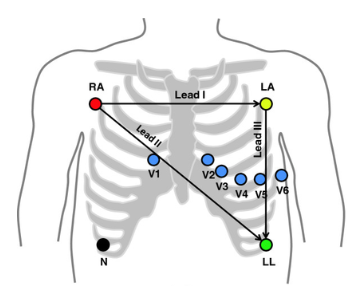
\includegraphics[scale=1]{lead.PNG}
\caption{ECG lead placement}
\label{fig:lead}
\end{figure}

\paragraph{} Annotations are loaded with the signal and the timestamp is converted from index position to a time value. PhysioNet annotations are converted to AAMI classes as in Table \ref{table:classes}\footnote{Description of PhysioNet annotations is available here https://archive.physionet.org/physiobank/annotations.shtml}. Annotations that do not correspond to heartbeats are removed. 

\begin{table}[h!]
\centering
\caption{MIT-BIH database information}
\label{table:database}
 \begin{tabular}{c|l|l} 
 \hline
 Value & Class & PhysioNet annotations \\
 \hline
 1 & N = any heartbeat not in S, V, F or Q & N, L, R, B, e, j, n\\
 2 & S = supraventricular ectopic beat & A, a, J, S\\
 3 & V = ventricular ectopic beat& V, r, E \\
 4 & F = fusion beat& F\\
 5 & Q = unknown or paced beat& /, f, Q\\
 -1 & Other annotation & \\
 \hline
 \end{tabular}
\end{table}

\paragraph{} If a resampling frequency is specified in the parameters, the database signal is interpolated (smooth spline approximation). 

\paragraph{} The output data is a 2xN array with approximated analog ECG signal in mV, float type, at 360Hz or specified resampling frequency. 

\section{Executing the model}
\paragraph{} The model takes as input a 2xN array with the ECG lead data (in mV) as provided by the database (cfr. Section \ref{section:open}. The model applies consecutively the AFE model on each lead. The digitized signal is then provided as input for the DBE model. The output consists in the detected beats with inferred label and time location, extracted feature vectors and estimated power consumption for AFE and DBE. 

\subsection{AFE model}
The AFE model approximates the effect of the IA and ADC separately on the ECG signal. The model works on one channel at a time. 

\paragraph{IA} The IA input-referred noise is first generated randomly with the sum of pink and white noise and added to the signal. The IA transfer function is applied, including distortion. Two signals are obtained at the output, corresponding to positive and negative terminals of the differential signal. 

\paragraph{ADC} The ADC input-referred noise is added similarly to the IA noise. The digitization is applied by first using the VCO transfer function to go from voltage to frequency domain, then integrating and quantizing and sampling the phase to obtain the digital output. 



\appendix

\section{MIT-BIH database information}
\label{section:database}
\paragraph{}Tables \ref{table:database} and \ref{table:database2} summarize the record information \footnote{Records 102, 104, 107 and 217 are skipped as they contain paced beats.}. 
\begin{sidewaystable}[h!]
\centering
\caption{MIT-BIH database information}
\label{table:database}
 \begin{tabular}{c|c|c|c|c|p{14cm}} 
 \hline
 Record & Length & Leads & Age & Sex & Info \\
 \hline
 100 & 30min & MLII + V5 & 69 & M & \\
 101 & 30min & MLII + V1 & 75 & F & \\
 103 & 30min & MLII + V2 & ? & M & \\
 105 & 30min & MLII + V1 & 73 & F & The PVCs are uniform.  The predominant feature of this tape is high-grade noise and artifact.\\
 106 & 30min & MLII + V1 & 24 & F & The PVCs are multiform.\\
 108 & 30min & MLII + V1 & 87 & F & There is borderline first degree AV block and sinus arrhythmia. The PVCs are multiform. The lower channel exhibits considerable noise and baseline shifts.\\
 109 & 30min & MLII + V1 & 64 & M & There is first degree AV block.  The PVCs are multiform.\\
 111 & 30min & MLII + V1 & 47 & F & There is first degree AV block.  There are short bursts of both baseline shifts and muscle noise, but in general, the quality is excellent.\\
 112 & 30min & MLII + V1 & 54 & M & There is S-T segment depression in the upper channel.\\
 113 & 30min & MLII + V1 & 24 & F & The variation in the rate of normal sinus rhythm is possibly due to a wandering atrial pacemaker.\\
 114 & 30min & MLII + V5 \footnote{Signals sometimes need to be reordered to have MLII first} & 72 & F & The PVCs are uniform.\\
 115 & 30min & MLII + V1 & 39 & F & \\
 116 & 30min & MLII + V1 & 68 & M & There are two PVC forms.\\
 117 & 30min & MLII + V2 & 69 & M & \\
 118 & 30min & MLII + V1 & 69 & M & The PVCs are multiform.\\
 119 & 30min & MLII + V1 & 51 & F & The PVCs are uniform.\\
 121 & 30min & MLII + V1 & 83 & F & \\
 122 & 30min & MLII + V1 & 51 & M & The lower channel has low-amplitude high-frequency noise throughout.\\
 123 & 30min & MLII + V5 & 63 & F & The PVCs are uniform and interpolated.\\
 124 & 30min & MLII + V4 & 77 & M & The PVCs are multiform. The junctional escape beats follow PVCs.\\
 200 & 30min & MLII + V1 & 64 & M & The PVCs are multiform. There are occasional bursts of high-frequency noise in the upper channel, and severe noise and artifact in the lower channel.\\
 201 & 30min & MLII + V1 & 68 & M & The PVCs are uniform and late-cycle. Junctional escape beats occur following episodes of ventricular trigeminy.\\
 202 & 30min & MLII + V1 & 68 & M & The PVCs are uniform and late-cycle. This record was taken from the same analog tape as record 201. \\
 203 & 30min & MLII + V1 & 43 & M & The PVCs are multiform. There are QRS morphology changes in the upper channel due to axis shifts. There is considerable noise in both channels, including muscle artifact and baseline shifts. This is a very difficult record, even for humans! \\
 205 & 30min & MLII + V1 & 59 & M & The PVCs are of two forms, one of which is much more common than the other.\\
 207 & 30min & MLII + V1 & 89 & F & This is an extremely difficult record. The predominant rhythm is normal sinus with first degree AV block and left bundle branch block. There are periods when the conduction block changes to a right bundle branch block pattern. The PVCs are multiform. Idioventricular rhythm appears following the longest episode of ventricular flutter. The record ends during the episode of SVTA.\\
 \hline
 \end{tabular}
\end{sidewaystable}

\begin{sidewaystable}[h!]
\centering
\caption{MIT-BIH database information (continued)}
\label{table:database2}
 \begin{tabular}{c|c|c|c|c|p{14cm}} 
 \hline
 Record & Length & Leads & Age & Sex & Info \\
 \hline
 208 & 30min & MLII + V1 & 23 & F & The PVCs are uniform. The couplets, many of which include a fusion PVC, are often seen in a bigeminal pattern. The triplets each consist of two PVCs and a fusion PVC.\\
 209 & 30min & MLII + V1 & 62 & M & \\
 210 & 30min & MLII + V1 & 89 & M & The PVCs are multiform.\\
 212 & 30min & MLII + V1 & 32 & F & There is rate-related right bundle branch block which appears when the heart rate exceeds approximately 90 bpm.\\
 213 & 30min & MLII + V1 & 61 & M & The PVCs are multiform and usually late-cycle, frequently resulting in fusion PVCs. The morphology of the fusion PVCs varies from almost normal to almost identical to that of the PVCs.\\
 214 & 30min & MLII + V1 & 53 & M & The PVCs are multiform. There are two episodes of artifactual amplitude decrease and one occurrence of tape slippage.\\
 215 & 30min & MLII + V1 & 81 & M & The PVCs are multiform. There are two very short occurrences of tape slippage (each less than one second in duration).\\
 219 & 30min & MLII + V1 & ? & M & Following some conversions from atrial fibrillation to normal sinus rhythm are pauses up to 3 seconds in duration. The PVCs are multiform.\\
 220 & 30min & MLII + V1 & 87 & F & \\
 221 & 30min & MLII + V1 & 83 & M & The PVCs are multiform, but one form is much more common than the others.\\
 222 & 30min & MLII + V1 & 84 & F & The episodes of paroxysmal atrial flutter/fibrillation are usually followed by nodal escape beats. There are several intervals of high-frequency noise/artifact in both channels.\\
 223 & 30min & MLII + V1 & 73 & M & The PVCs are multiform. The two longest episodes of ventricular tachycardia are slow (100 to 105 bpm) and bidirectional.\\
 228 & 30min & MLII + V1 & 80 & F & There is first degree AV block.  The PVCs are multiform. There are three short occurrences of tape slippage with a maximum duration of 2.2 seconds.\\
 230 & 30min & MLII + V1 & 32 & M & \\
 231 & 30min & MLII + V1 & 72 & F & AV conduction is quite abnormal with periods of 2:1 AV block, examples of Mobitz II block, and right bundle branch block which appears to be rate-related.  The couplet is probably ventricular.\\
 232 & 30min & MLII + V1 & 76 & F & The rhythm is compatible with sick sinus syndrome. There is underlying sinus bradycardia, first degree AV block, and frequent ectopic atrial runs at rates of 80 to 90 bpm. There are numerous long pauses up to 6 seconds in duration.\\
 233 & 30min & MLII + V1 & 57 & M & The PVCs are multiform.\\
 234 & 30min & MLII + V1 & 56 & F & The PVCs are uniform.\\
 
 \hline
 \end{tabular}
\end{sidewaystable}

\end{document}
